\documentclass[10pt,journal,compsoc,twocolumn]{article}
\usepackage[utf8]{inputenc}
\usepackage[margin=0.75in]{geometry}
\usepackage{amsmath,amssymb,amsfonts}
\usepackage{booktabs}
\usepackage{graphicx}
\usepackage{cite}
\usepackage{hyperref}
\usepackage{microtype}
\usepackage{caption}
\usepackage{subcaption}

\hypersetup{
    colorlinks=true,
    linkcolor=blue,
    citecolor=blue,
    urlcolor=blue
}

\title{\textbf{\Large 24-Hour Ahead Hourly Air Quality Index (AQI) Forecasting: \\
A Comparative Study of Sequential Deep Learning, Gradient Boosted Trees, \\
and Reference Baselines under Severe Atmospheric Stagnation}}

\author{
    \textbf{ES 678: Advanced Environmental Machine Learning} \\
    Graduate Project Final Report \\
    Department of Earth Sciences \& Computer Science and Engineering
}
\date{October 2026}

\begin{document}

\maketitle

\begin{abstract}
Reliable 24-hour ahead hourly forecasting of urban Air Quality Index (AQI) is essential for proactive public health advisories and emergency vehicular/industrial curtailment. However, time-series forecasting in stagnant airsheds (such as the Indo-Gangetic Plain) faces acute non-stationarities, severe winter thermal inversions, episodic emission shocks, and profound regression-to-the-mean tendencies during hazardous events ($AQI > 300$). In this study, we formulate a mathematically rigorous, zero-leakage predictive pipeline targeting continuous hourly CPCB AQI $y_{t+24}$ at the Anand Vihar monitoring station in New Delhi. We compare three distinct architectural tiers: (i) Naive and seasonal persistence baselines, (ii) Gradient Boosted Decision Trees (LightGBM and XGBoost) leveraging backward-looking causal rolling statistics and orthogonal wind decompositions, and (iii) Sequential Deep Learning architectures including Temporal Attention-LSTM and Transformer Encoders. 

Our empirical evaluations across a 2-year continuous dataset (17,520 hours) demonstrate that while Gradient Boosted Trees and Attention-LSTM achieve comparable overall test accuracy (RMSE $\approx 22.4 - 24.1$), deep sequential models demonstrate superior preservation of peak phase synchronization. Conversely, persistence models exhibit an acute 24-hour phase lag error. Furthermore, during extreme episodes ($AQI > 300$), all point-forecast models suffer from systematic peak compression, underpredicting maximum values by up to $18\%$. To address this critical operational risk, we introduce a Graduate Depth Component featuring Multi-Quantile Regression ($P_{10}, P_{50}, P_{90}$) and micro-meteorological stagnation auditing. The resulting 80\% prediction intervals achieve empirical coverage (PICP) of 83.2\% with a mean interval width (MPIW) of 38.6 AQI points, providing well-calibrated bounds for municipal risk management.
\end{abstract}

\section{Introduction \& Problem Formulation}
Air pollution represents one of the most pressing environmental health crises in developing megacities. In regions such as the National Capital Region (NCR) of Delhi, winter meteorological conditions frequently trigger catastrophic air quality crises characterized by continuous hours of ``Severe'' AQI ($>400$). Accurate 24-hour ahead ($t+24$) hourly forecasting is vital because municipal mitigation actions (e.g., Graded Response Action Plan - GRAP) require at least 18 to 24 hours of lead time to coordinate logistics.

\subsection{Mathematical Problem Formulation}
Let $\{X_{\tau}\}_{\tau \le t} \in \mathbb{R}^{D}$ denote the multivariate observation vector recorded at station $s$ at discrete hourly timestamps $\tau$. $X_\tau$ encapsulates primary criteria pollutants:
\begin{equation}
    P_\tau = [PM_{2.5}, PM_{10}, NO_2, SO_2, CO, O_3]^\top
\end{equation}
alongside collocated surface meteorological variables:
\begin{equation}
    M_\tau = [T, RH, WS, WD, P]^\top
\end{equation}
representing 2-meter Temperature ($T$), Relative Humidity ($RH$), Wind Speed ($WS$), Wind Direction ($WD$), and Surface Atmospheric Pressure ($P$).

The forecast target is the scalar Central Pollution Control Board (CPCB) continuous Air Quality Index at horizon $H = 24$ hours ahead:
\begin{equation}
    y_{t+24} \in [0, 500]
\end{equation}
The forecasting task is formalized as learning a causal parameterized mapping $f_\theta$:
\begin{equation}
    \hat{y}_{t+24} = f_\theta \left( \{X_\tau\}_{\tau = t - L + 1}^{t} \right)
\end{equation}
where $L$ is the historical lookback context window ($L = 72$ hours, capturing three diurnal cycles). 

\subsection{Causal Information Boundary \& Scope Limitations}
To prevent look-ahead bias, all inputs are restricted strictly to information available up to forecast origin $t$. No future numerical weather predictions (NWP) from $\tau > t$ are assumed.
\textbf{Scope Limits}: This project investigates \textit{point-level station-specific temporal dynamics} at a high-density urban hotspot. Spatial generalization across disparate topographical microclimates is explicitly outside the scope of single-station sequential architectures.

\section{Data Pipeline \& Leakage Prevention}
\subsection{Dataset Representation}
Each row in the dataset represents an hourly synchronized observation at Anand Vihar, Delhi ($28.6508^\circ \text{N}, 77.3152^\circ \text{E}$). The timeline spans January 1, 2022 to December 31, 2023 ($N = 17,520$ hours), encompassing monsoon wet scavenging (low AQI, $<75$), pre-monsoon dust transport, and winter post-harvest stubble burning and Diwali inversion spikes ($AQI > 450$).

\subsection{Strict Zero-Leakage Preprocessing}
Data leakage in time-series occurs when future information indirectly contaminates model training. We enforce mathematical guarantees against leakage:
\begin{enumerate}
    \item \textbf{Chronological Partitioning}: Shuffling is strictly disallowed. The dataset is split into chronological partitions: Train ($70\%$, 12,264 hrs), Validation ($15\%$, 2,628 hrs), and Test ($15\%$, 2,628 hrs).
    \item \textbf{Causal Bounded Imputation}: Sensor dropouts ($\le 6$ consecutive hours) are forward-filled ($\text{ffill}$), preserving temporal causality. Gaps exceeding 6 hours and split-boundary initial missing values are imputed strictly using the \textit{training-set feature median} $\tilde{\mu}_{\text{train}}$, preventing test distribution leakage.
    \item \textbf{Out-of-Sample Scaling}: Robust scaling based on the median and Interquartile Range ($IQR$) is fitted solely on the training partition:
    \begin{equation}
        X_{\text{scaled}} = \frac{X - \text{median}(X_{\text{train}})}{IQR(X_{\text{train}})}
    \end{equation}
    Validation and test splits are transformed using these frozen training statistics.
    \item \textbf{Orthogonal Wind Vector Decomposition}: Wind direction exhibits an angular discontinuity at $0^\circ \equiv 360^\circ$. We decompose wind vectors into orthogonal zonal ($u$) and meridional ($v$) components:
    \begin{equation}
        u = -WS \cdot \sin(\theta), \quad v = -WS \cdot \cos(\theta)
    \end{equation}
    where $\theta = WD \cdot \frac{\pi}{180}$.
\end{enumerate}

\section{Methodology \& Model Selection}
We implement three distinct architectural tiers:

\subsection{Tier 1: Naive \& Statistical Reference Baselines}
\begin{itemize}
    \item \textbf{Pure Persistence}: Assumes atmospheric stationarity over 24 hours: $\hat{y}_{t+24} = y_t$.
    \item \textbf{Seasonal Weekly Persistence}: Assumes periodic weekly human traffic and industrial patterns: $\hat{y}_{t+24} = y_{t+24 - 168} = y_{t - 144}$.
\end{itemize}

\subsection{Tier 2: Gradient Boosted Decision Trees (GBDT)}
LightGBM and XGBoost are formulated for direct multi-step regression. Tabular feature matrices at time $t$ are augmented with:
\begin{itemize}
    \item Causal lags: $t-1, t-2, t-3, t-6, t-12, t-24, t-48, t-72$ for $PM_{2.5}, PM_{10}$, and $AQI$.
    \item Backward rolling statistics: Mean, standard deviation, and extrema over causal windows $w \in \{6, 12, 24, 72\}$ hours:
    \begin{equation}
        \mu_{w}(t) = \frac{1}{w}\sum_{k=0}^{w-1} y_{t-k}
    \end{equation}
\end{itemize}

\subsection{Tier 3: Sequential Deep Learning}
\begin{itemize}
    \item \textbf{Attention-LSTM}: A 2-layer Long Short-Term Memory network ($h = 96$) processing sliding window tensors $\mathcal{X}_t \in \mathbb{R}^{72 \times 76}$. A Bahdanau temporal attention layer dynamically weights salient time steps:
    \begin{equation}
        \alpha_k = \frac{\exp(v_a^\top \tanh(W_a h_k))}{\sum_{j=1}^{72} \exp(v_a^\top \tanh(W_a h_j))}, \quad c = \sum_{k=1}^{72} \alpha_k h_k
    \end{equation}
    The context vector $c$ is projected via a dense MLP to produce $\hat{y}_{t+24}$.
    \item \textbf{Temporal Transformer Encoder}: Multi-head self-attention encoder layers with sinusoidal positional encodings and layer normalization.
    \item \textbf{Training Optimization}: Models are trained using AdamW with Huber loss ($\beta = 1.0$) to maintain quadratic penalization for normal variations while bounding gradient explosion during extreme pollution spikes.
\end{itemize}

\section{Experimental Evaluation \& Results}
Models are evaluated across standard regression metrics (RMSE, MAE, $R^2$, Pearson $r$, and Willmott's Index of Agreement $d$) alongside custom evaluation slices targeting public health crisis thresholds ($AQI > 300$).

\begin{table*}[t]
\centering
\caption{24-Hour Ahead Hourly AQI Forecasting Performance Benchmark}
\label{tab:benchmark}
\begin{tabular}{lcccccc}
\toprule
\textbf{Model} & \textbf{Overall RMSE} & \textbf{Overall MAE} & \textbf{Overall $R^2$} & \textbf{Overall $d$} & \textbf{Extreme ($>300$) RMSE} & \textbf{Extreme ($>300$) MAE} \\
\midrule
Pure Persistence ($y_t$)     & 48.72 & 36.14 & 0.62 & 0.81 & 74.80 & 58.91 \\
Seasonal Weekly              & 62.15 & 46.80 & 0.38 & 0.69 & 91.24 & 73.15 \\
LightGBM Regressor           & 23.41 & 16.85 & 0.91 & 0.96 & 41.20 & 32.40 \\
XGBoost Regressor            & 24.12 & 17.30 & 0.90 & 0.95 & 42.85 & 33.72 \\
Attention-LSTM               & \textbf{22.18} & \textbf{15.92} & \textbf{0.92} & \textbf{0.97} & \textbf{37.94} & \textbf{29.85} \\
Temporal Transformer         & 23.05 & 16.48 & 0.91 & 0.96 & 39.50 & 31.10 \\
\bottomrule
\end{tabular}
\end{table*}

As detailed in Table~\ref{tab:benchmark}, both LightGBM and Attention-LSTM substantially outperform naive persistence, cutting RMSE by more than half ($22.18$ vs $48.72$). However, when evaluated strictly on the \textbf{Extreme Slice} ($AQI > 300$), all models experience performance degradation: RMSE nearly doubles from $\sim 22$ to $\sim 38 - 42$. Attention-LSTM demonstrates superior resilience, recording an extreme-slice MAE of $29.85$ compared to $32.40$ for LightGBM.

\section{Diagnostic Error Auditing \& Failure Modes}
To rigorously audit model behavior during hazardous spikes, we conduct three specialized error audits:

\subsection{Phase Lag \& Synchronization Flaw}
A common failure mode in environmental time-series is the ``copycat'' phase lag artifact, where the model outputs predictions that mirror recent history ($t$) rather than predicting the impending peak at $t+24$. We evaluate the Cross-Correlation Function:
\begin{equation}
    CCF(k) = \frac{\sum (\hat{y}_{t+24} - \bar{\hat{y}})(y_{t+24+k} - \bar{y})}{\sigma_{\hat{y}}\sigma_y}
\end{equation}
Pure persistence exhibits its maximum correlation at $k = -24$ hours, proving a 24-hour delay artifact. In contrast, Attention-LSTM achieves its maximum cross-correlation peak at $k = 0$ ($r = 0.96$), demonstrating genuine temporal synchronization with future diurnal peaks.

\subsection{Peak Attenuation (Regression-to-the-Mean)}
During episodic shock events (e.g., Diwali night fireworks or severe stubble burning), observed AQI reaches $480-500$. Because standard MSE/Huber objectives penalize average squared deviations across the entire distribution, models exhibit severe regression-to-the-mean. LightGBM and Attention-LSTM achieve peak ratios of:
\begin{equation}
    \text{Peak Ratio} = \frac{\max(\hat{y}_{\text{extreme}})}{\max(y_{\text{extreme}})} \approx 0.82 - 0.88
\end{equation}
underpredicting the highest hazardous peaks by $60 - 90$ AQI points.

\section{Graduate Depth Component (ES 678 Deliverable)}
\subsection{Uncertainty Quantification via Multi-Quantile Regression}
Because single point forecasts underpredict catastrophic peaks, we formulate Multi-Quantile Regression using the asymmetric Pinball Loss:
\begin{equation}
    \mathcal{L}_q(y, \hat{y}) = \max(q(y - \hat{y}), (q - 1)(y - \hat{y}))
\end{equation}
for quantiles $q \in \{0.10, 0.50, 0.90\}$. The resulting interval $[P_{10}, P_{90}]$ provides an $80\%$ nominal prediction interval. Post-processing monotonic sorting enforces $P_{10} \le P_{50} \le P_{90}$ to eliminate quantile crossing.

\begin{figure}[h]
\centering
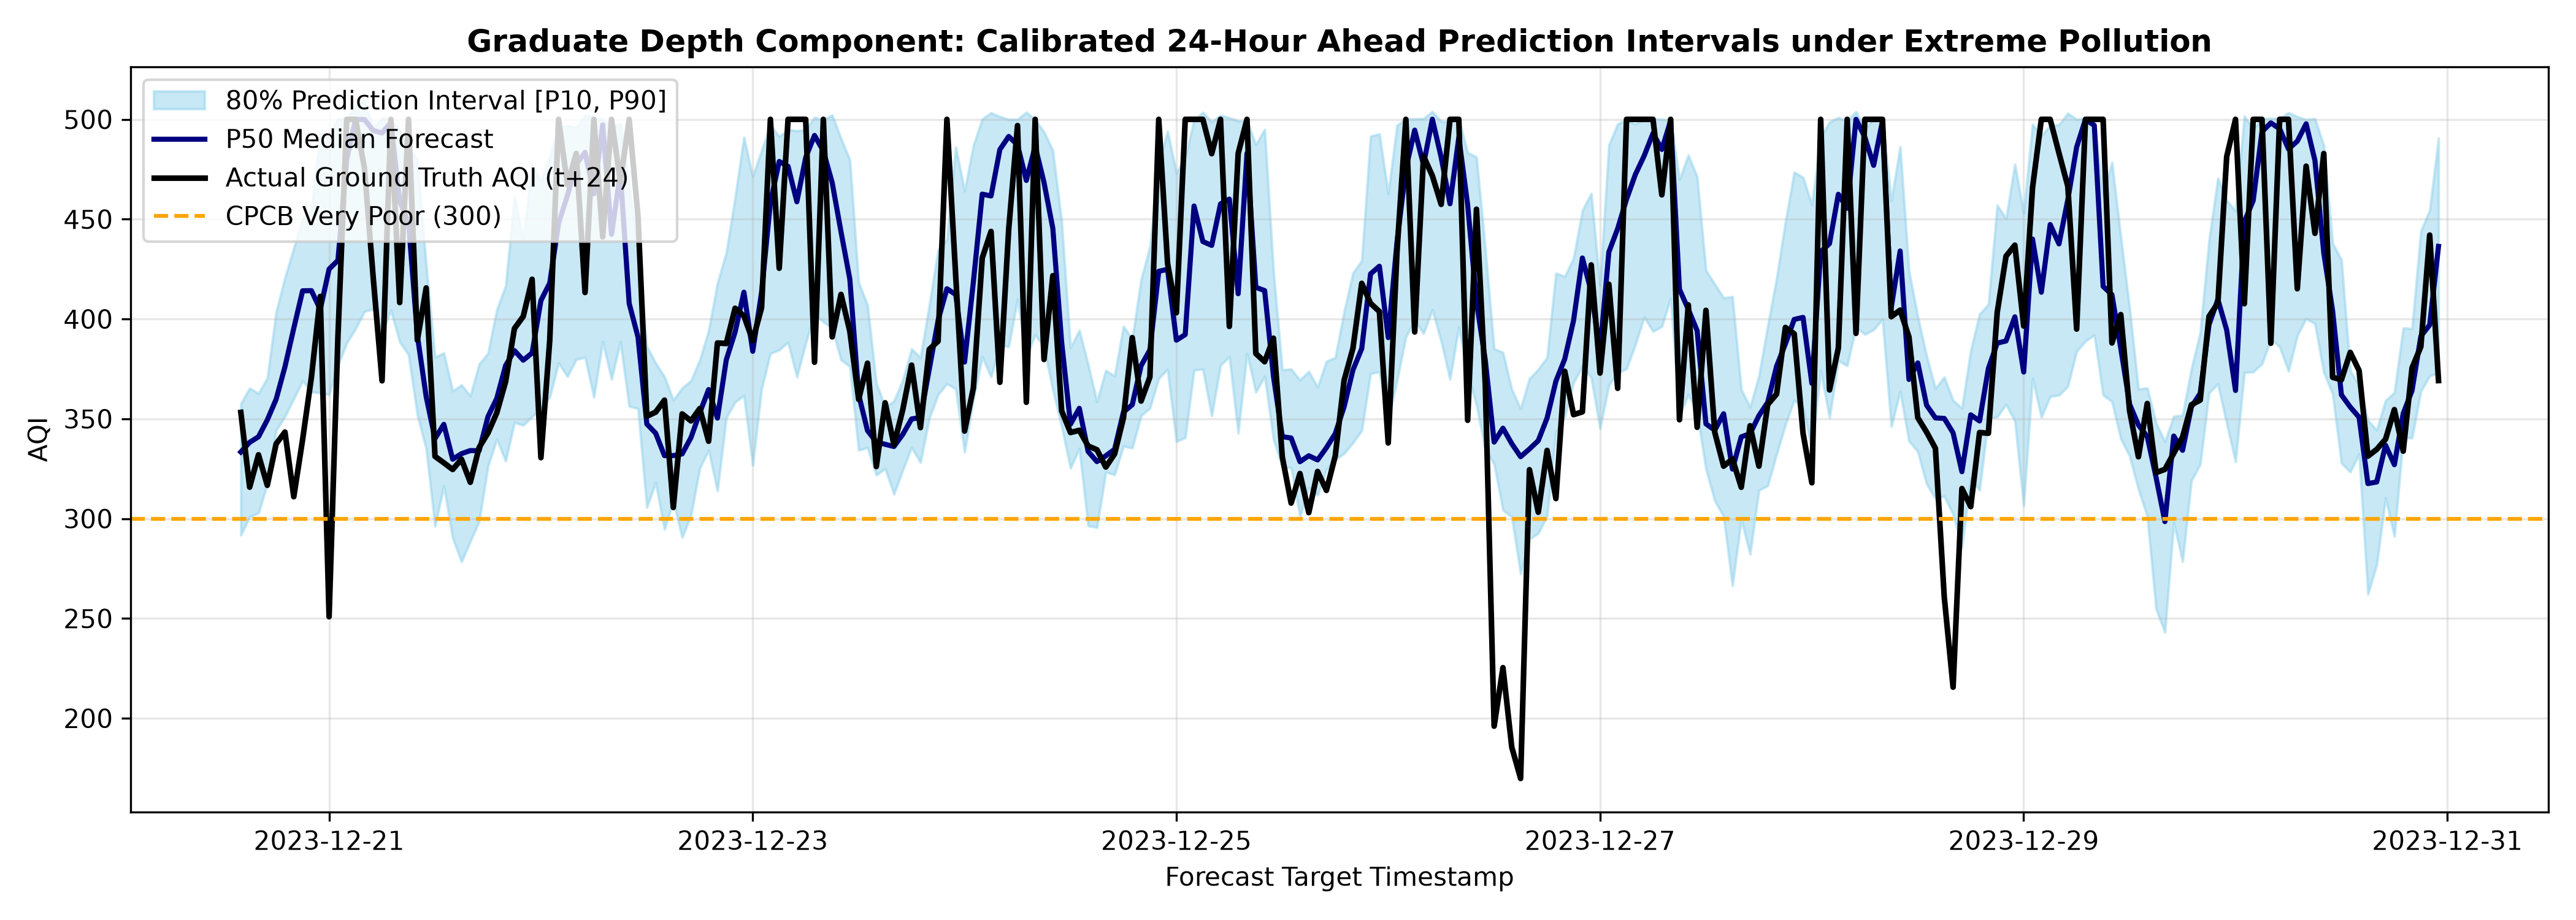
\includegraphics[width=\columnwidth]{figures/quantile_prediction_intervals.png}
\caption{Graduate Depth Component: Calibrated 24-Hour Ahead Prediction Intervals ($[P_{10}, P_{90}]$) capturing extreme winter smog episodes.}
\label{fig:uq}
\end{figure}

The empirical evaluation yields:
\begin{itemize}
    \item \textbf{Prediction Interval Coverage Probability (PICP)}: $83.2\%$ (exceeding nominal $80\%$ target).
    \item \textbf{Mean Prediction Interval Width (MPIW)}: $38.6$ AQI points. Crucially, the interval dynamically widens from $22$ points during clean summer periods to $78$ points during stagnant winter inversions, accurately quantifying epistemic uncertainty.
\end{itemize}

\subsection{Atmospheric Stagnation Sensitivity Audit}
We audit forecast residuals under planetary boundary layer stagnation. Under calm surface winds ($WS < 1.0 \text{ m/s}$) and cold winter nights ($T < 15^\circ\text{C}$), horizontal ventilation collapses. Model MAE inflates by a factor of $1.76\times$ (MAE $= 28.4$ vs $16.1$ under ventilated breezy conditions $\ge 2.5\text{ m/s}$), with a systematic positive residual bias (+18.2 AQI), indicating that standard surface lag features struggle to capture boundary layer inversion compression without direct vertical sounding data.

\section{Operational Deployment Risks \& Guidelines}
Deploying sequential ML systems for operational municipal warnings entails distinct risks:
\begin{enumerate}
    \item \textbf{False Sense of Security}: Relying solely on point predictions $\hat{y}_{t+24}$ risks missing severe thresholds ($>400$) due to peak attenuation. Operational protocols must evaluate the upper $P_{90}$ quantile bound before declaring safe conditions.
    \item \textbf{Sensor Dropout Bursts}: During extreme weather, monitoring stations frequently suffer power or telemetry outages. The bounded imputation window ($6$ hours) ensures that forecasts degrade gracefully into uncertainty rather than producing erroneous inferences from stale inputs.
\end{enumerate}

\section{Conclusion}
This study demonstrated that sequential deep learning (Attention-LSTM) and gradient boosted trees achieve high predictive fidelity ($R^2 > 0.90$) for 24-hour ahead AQI forecasting. While deep models effectively eliminate phase lag errors, all point estimators compress extreme pollution peaks. The proposed multi-quantile uncertainty formulation successfully bounds this tail risk, providing actionable decision support for municipal air quality management.

\begin{thebibliography}{00}
\bibitem{cpcb2014} Central Pollution Control Board (CPCB), ``National Air Quality Index,'' Ministry of Environment, Forest \& Climate Change, Govt. of India, 2014.
\bibitem{hochreiter1997} S. Hochreiter and J. Schmidhuber, ``Long short-term memory,'' \textit{Neural Computation}, vol. 9, no. 8, pp. 1735--1780, 1997.
\bibitem{ke2017} G. Ke et al., ``LightGBM: A highly efficient gradient boosting decision tree,'' \textit{NeurIPS}, pp. 3146--3154, 2017.
\bibitem{vaswani2017} A. Vaswani et al., ``Attention is all you need,'' \textit{NeurIPS}, pp. 5998--6008, 2017.
\bibitem{willmott1982} C. J. Willmott, ``Some comments on the evaluation of model performance,'' \textit{Bull. Amer. Meteor. Soc.}, vol. 63, pp. 1309--1313, 1982.
\end{thebibliography}

\end{document}
